%Bayesianizing conditional distribution
% The conditional distribution $p(y|x)$ obtained from using a Gaussian mixture model is without a prior, and
% the predictive distribution yields a way too small uncertainty estimate in regions where there are no observations.
% This is because the range of the Gaussian distribution continues throughout the entire space and even though the
% joint distribution is very small in the region, the conditional distribution is normalized using the (very small) $p(x)$.
% We, therefore, want to introduce a prior, which can rule over the conditional in regions where the probability is too
% small. The first approach is simply to define a new conditional distribution, 

As mentioned above the conditional itself is not enough as a probabilistic regression model used as
a surrogate model. This is showcased in the middle right illustration in Figure
\ref{pred_dist_manipulation}, where the conditional distribution would have the same distance
between its confidence bounds even for those $x$ far away. To our knowledge, this problem has not
been dealt with in the literature before. We want to manipulate the conditional distribution to 
transform into a very uncertain prior probability for $y$ in areas
where there is small evidence of the data $p(x)$. Two of the ideas for manipulating the conditional distributions
(denoted $\hat p(y|x)$), %This opens up a wide range of ideas:
\begin{enumerate}
    \item Include a new Gaussian mixture component with zero mean and large variance, $p_{prior}(y)$, and 
    choose an $x$-depended weighting, $\alpha_x \in [0,1]$, such that $$\hat p(y|x) = \alpha_x p(y|x) + (1-\alpha_x)p_{prior}(y)$$
    \item Assuming both the conditional and prior distribution to be a Gaussian, we could choose an-$x$ 
    depended weighting, $\alpha_x \in [0,1]$ such that the manipulate conditional is a Gaussian with mean
    $\hat\mu$ and variance $\hat \sigma^2$ such that, 
    \begin{align*}
        \hat \mu &:= \alpha_x \cdot \mu_{y|x} + (1-\alpha_x) \cdot \mu_{prior}\\
        \hat \sigma^2 &:= \alpha_x \cdot \sigma_{y|x}^2 + (1-\alpha_x) \cdot\sigma_{prior}^2
    \end{align*}
\end{enumerate}

We define $x$-depending weighting to be a function of the evidence $p(x)$ and how much data is observed $N$,
and we additionally introduce a parameter $\Delta>0$,
$$\alpha_x = \frac{N\cdot p(x)\cdot \Delta}{N\cdot p(x)\cdot \Delta+1}$$
note that $\alpha_x = 0$ for $p(x) = 0$ and $\alpha_x \rightarrow 1$ for $N\cdot p(x)\cdot \Delta \rightarrow \infty$. 
Illustration of idea 1 can be seen in left illustration in Figure \ref{pred_dist_manipulation} where we call
$S(x) := N\cdot p(x)\cdot \Delta$ the scaling. 

Idea 1 would work on any kind of conditional distribution, while idea 2 would be an intuitive transformation
but only if the conditional is Gaussian, or alternative, as we are working with mixtures 
of Gaussians, these could be manipulated in the same way. 

% \begin{tcolorbox}[
%     sharp corners,
%     boxrule=0mm,
%     enhanced,
%     borderline west={4pt}{0pt}{gray},
%     colframe=drGray,
%     colback=drGray,
%     coltitle=black,
% ]
% {\large \textbf{Note: Idea 1 defines a valid distribution}}\\
%     The manipulated conditional in idea 1, is a convex combination of valid distributions, 
%     and it is always positive and integrates to 1, as easily seen here, 
%     \begin{align*}
%         \int_y \hat p(y|x) dy &= \int_y \left[ \alpha_x p(y|x) + (1-\alpha_x)p_{prior}(y) \right] dy\\
%         &= \alpha_x \int_y p(y|x)dy +(1-\alpha_x) \int_y p_{prior}(y)dy \\
%         &= \alpha_x + (1-\alpha_x) = 1.
%     \end{align*}
% \end{tcolorbox}

% In figure \ref{pred_dist_manipulation} the manipulated predictive 
% distribution is illustrated under the influenced of different scalings. 
% Note that if $S(x) = 0$ the manipulated distribution becomes the prior,
% while in the limit $S(x) \rightarrow \infty$ the manipulated distribution
% become the original predictive distribtuion, $\hat p(y|x) = p(y|x)$. 

\begin{figure}[H]
    \centering
    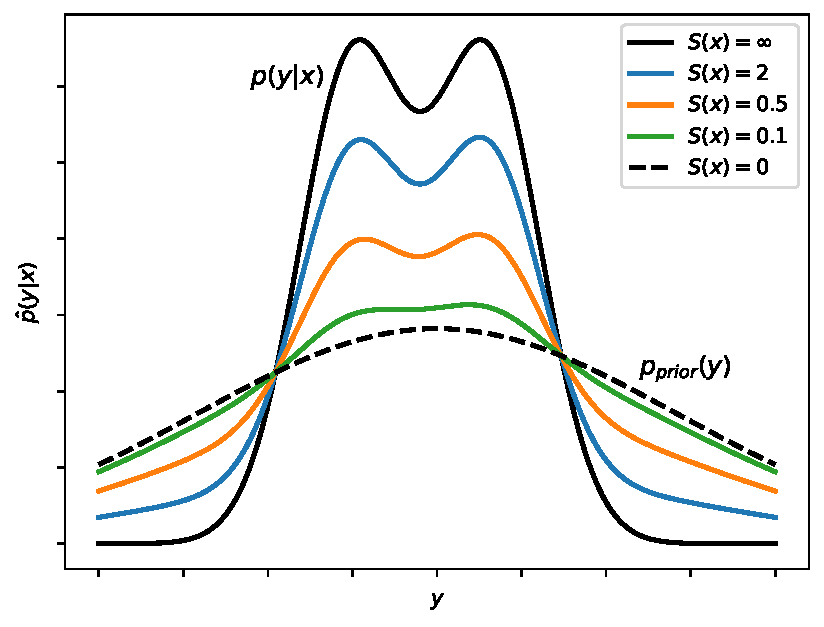
\includegraphics[trim=0.3cm 0cm 0.1cm 0.2cm,clip,width=0.49\textwidth]{Pictures/mixture_predictive_bayesian.pdf}
    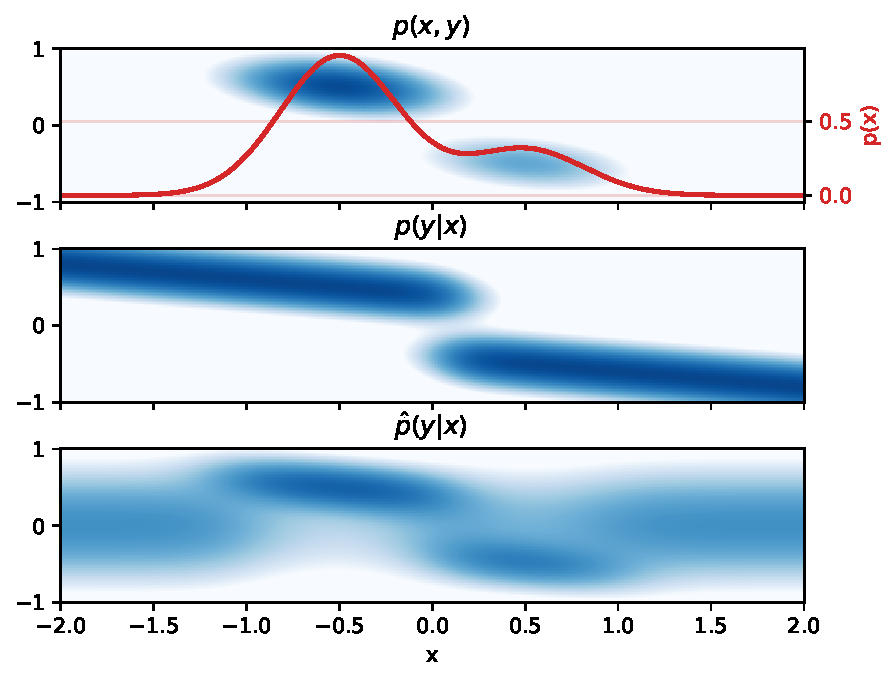
\includegraphics[trim=0.3cm 0cm 0.1cm 0.2cm,clip,width=0.49\textwidth]{Pictures/mixture_predictive_bayesian2D.pdf}
    \caption{Left: Illustration of how the preditive distribution is manipulated according
    the the scaling function $S(x) := p(x)\cdot N\cdot \Delta$. Right: Illustration of why it makes
    sense to manipulate the predictive distribution $p(y|x)$, if there is a small amount of input data
    at a region, then the predictive distribution should transform into the uncertain prior}
    \label{pred_dist_manipulation}
\end{figure}

\subsection{Mean and variance of predictive distribution}\label{mean_variance_pred_mixture}
If we just are interested in a Gaussian approximation of the predictive
distribution, this can be easily done assuming we know the mean, variance
and the second moment of the conditional distribution, first the predictive mean
is calculate, 
\begin{align*}
    \mathbb{E}_{\hat p(y|x)}[y] &= \int y \cdot \left(\alpha_x \cdot p(y|x) + (1-\alpha_x) p_{prior}(y)\right) dy\\
    &= \alpha_x\cdot \mathbb{E}_{p(y|x)}[y] + (1-\alpha_x)\cdot \mathbb{E}_{p_{prior}(y)}[y]
\end{align*}

And the predictive variance is calcualted, using the definition of variance, $\mathbb{V}_{\hat p(y|x)}[y] =
\mathbb{E}_{\hat p(y|x)}[y^2] - \mathbb{E}_{\hat p(y|x)}[y]^2$. So we only need to calculate the second moment, 
\begin{align*}
    \mathbb{E}_{\hat p(y|x)}[y^2] &= \int y^2 \cdot \alpha_x \cdot p(y|x) + (1-\alpha_x) p_{prior}(y) dy\\
    &=\alpha_x \cdot \mathbb{E}_{p(y|x)}[y^2] +(1-\alpha_x) \cdot \mathbb{E}_{p_{prior}(y)}[y^2] \\
    &=\alpha_x \cdot(\mathbb{V}_{p(y|x)}[y]+\mathbb{E}_{p(y|x)}[y]^2) + (1-\alpha_x) \mathbb{V}_{p_{prior}(y)}[y]
\end{align*}
Assuming $\mathbb{E}_{p_{prior}(y)}[y] = 0$. 

\begin{note2}[Implementation]
    If we use $\alpha_x \propto p(x)$, then it is not necessary to calculate the conditional
    distribution at all. Assuming $c$ is a constant in $y$,
    $$\hat p(y|x) = \frac{c\cdot p(x)\cdot  p(y|x) + p_{prior}(y)}{c\cdot p(x)+1} = \frac{c \cdot p(x,y) + p_{prior}(y)}{c\cdot p(x)}.$$
\end{note2}

